\section{Background}
\label{sec:background}

In this section we briefly describe the necessary background to understanding key components of the \sysName system.
\subsection{Probabilistic Databases}

A \textit{probabilistic database} $\mathcal{DB}^{p}$ consists of two key components: (1) a collection of incomplete relations $\mathcal{R}$ with missing or uncertain data, and (2) a probability distribution $F$ on all possible database instances.  These \textit{possible worlds} denoted by pwd($DB^{p}$) represent multiple viable instances of the database.  The attributes of an incomplete relation $R \in \mathcal{R}$ may contain deterministic attributes, but also include a subset that are \textit{probabilistic attributes} $\mathcal{A}^{p}$.  The values of $\mathcal{A}^{p}$ may be present, missing, or uncertain.  Each possible database instance is a completion of the missing or uncertain data in $\mathcal{R}$.

\subsection{Conditional Random Fields (CRF)}
\label{sec:pi-crf}
\begin{figure}
        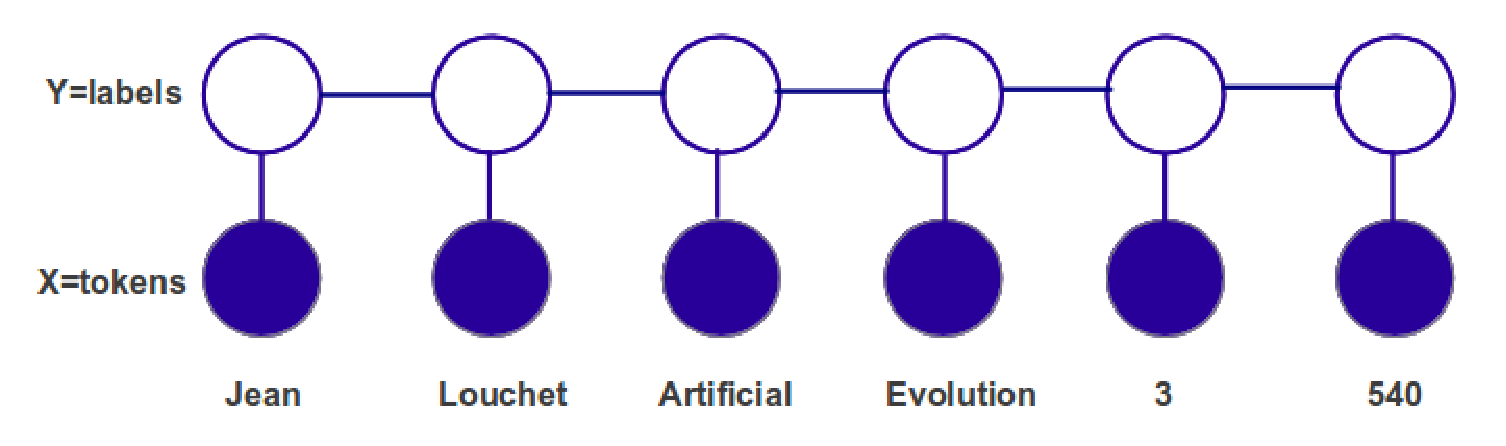
\includegraphics[width=0.9\textwidth]{CRF.eps}
        \caption{Example CRF model.}
        \label{fig:CRF}
\end{figure}

The linear-chain CRF~\cite{DBLP:conf/icml/LaffertyMP01,sutton06introduction}, an extension of the hidden Markov model, is a state-of-the-art probabilistic graphical model for solving IE tasks.  In the context of IE, a CRF model encodes the probability distribution over a set of \textit{label} random variables $y \in \mathbf{Y}$, given the value of a set of \textit{token} random variable $x \in \mathbf{X}$.  Assignments to $\mathbf{X}$ are given by $\mathbf{x}$ and to $\mathbf{Y}$ by $\mathbf{y}$.  In a linear-chain CRF model, label $y_{i}$ is correlated only with the previous label $y_{i-1}$ and the corresponding token $x_{i}$.  The set of these correlations $k \in K$ are represented by the feature functions $\{f_{k}(y_{i},y_{i-1},x_{i})\}^{K}_{k=1}$.

\begin{example}
Figure~\ref{fig:CRF} shows an example CRF model over a subset of the citation string from Example~\ref{ex:citation}.  Observed (known token) variables are shaded nodes in the graph.  Hidden (unknown label) variables are unshaded.  Edges in the graph denote statistical correlations.  For citations, the possible labels are $Y = \{$title, author, conference, isbn, publisher, series, proceedings, year\}.  Two possible feature functions of this CRF are:
\begin{align*}
    \centering
    f_{1}(y_{i}, y_{i-1}, x_{i}) &= [x_{i} \text{ appears in a conf list}] \cdot [y_{i} = \text{ conf}]\\
    f_{1}(y_{i}, y_{i-1}, x_{i}) &= [y_{i} = \text{ author}] \cdot [y_{i-1} = \text{ title}]
\end{align*}
\end{example}
Let $\{f_{k}(y_{i},y_{i-1},x_{i})\}^{K}_{k=1}$ be a set of real-valued feature functions, and $\Lambda = \{\lambda_{k}\} \in R^{K}$ be a vector of real-valued parameters, a CRF model defines the probabilistic distribution of segmentations $\mathbf{y}$ given a specific token sequence $\mathbf{x}$:
\begin{equation}
\label{eq:CRFmodel}
p(\mathbf{y} | \mathbf{x}) = \frac{1}{Z}\text{exp}\{\sum_{i=1}^{T}\sum_{k=1}^{K}\lambda_{k}f_{k}(y_{i},y_{i-1},x_{i})\},
\end{equation}
where $Z$ is a standard partition function that guarantees probability values between $0$ and $1$.

\subsection{Inference Queries over a CRF Model}
\newcommand{\topk}{top-\textit{k}\xspace}
There are three types of inference queries used in \sysName .

\textbf{Top-k Inference}: The \topk inference computes the segmentations with the \topk highest probabilities given a token sequence $\mathbf{x}$ from a text-string $d$.  The Viterbi dynamic programming algorithm~\cite{Viterbi1973} is the key algorithmic technique for CRF \topk inference.

%The Viterbi algorithm computes a two-dimensional V matrix, where each cell $V(i,y)$ stores a ranked list of \textit{entries} $e=\{score,$ $prev(label,idx)\}$ ordered by a \textit{score}.  Each entry contains (1) the \textit{score} of a \topk (partial) segmentation ending at position $i$ with label $y$; and (2) a pointer to the previous entry \textit{prev} on the path that led to the \topk \textit{score's} in $V(i,y)$.  The pointer $\text{e.prev}$ consists of the label $label$ and the list index $idx$ of the previous entry on the path to $e$.  Based on equation~\ref{eq:CRFmodel}, the recurrence to compute the ML (top-1) segmentation is as follows:
%\begin{equation}
%V(i,y) = \left\{
%\begin{array}{l l}
%\text{max}_{y'}(V(i-1,y')\\
%   + \sum_{k=1}^{K}\lambda_{k}f_{k}(y,y',x_{i})), & \quad \text{if } i \geq 0\\
%0, & \quad \text{if } $i$ = -1
%\end{array} \right.
%\end{equation}
%\eat{
%The ML segmentation $y*$, backtracked from the maximum entry in $V(T,y_{T})$ (where $T$ is the length of the token sequence \textbf{x}) through $\text{prev}$ pointers is shown in Figure~\ref{}.  }
%The complexity of the Viterbi algorithm is $O(T \cdot |L|^{2})$, where $|L|$ is the number of possible labels.

\textbf{Constrained Top-k Inference}: Constrained \topk inference~\cite{Kristjansson:2004:IIE:1597148.1597216} is a special case of traditional \topk inference.  It is used when a subset of the token labels has been provided (e.g., via a user interface such as Amazon Mechanical Turk).  Let $\mathbf{s}$ be the evidence vector $\{s_{1}, \dots, s_{T}\}$, where $s_{i}$ is either NULL (i.e., no evidence) or the evidence label for $y_{i}$.  Constrained \topk inference can be computed for a variant of the Viterbi algorithm which restricts the chosen labels $\mathbf{y}$ to conform to the evidence $\mathbf{s}$.

\textbf{Marginal Inference}: Marginal inference computes a marginal probability $p(y_{t},y_{t+1}, \dots, y_{t+k}|\mathbf{x})$ over a single node's label or a sub-sequence of nodes~\cite{sutton06introduction}.  The Forward-Backward algorithm, a variation of the Viterbi algorithm is used for such marginal inference tasks.  In \sysName, marginal inference is primarily employed over a single node corresponding to the marginal label distribution for individual tokens. 

%\subsection{Uncertainty Sampling}
%\label{sec:uncertainty}
%Uncertainty sampling has a long history in pool-based active learning~\cite{Lewis94heterogeneousuncertainty} and seeks to optimally select a set of unlabeled examples for labeling by experts.  The approach selects those that are the "least certain," which means they have the highest variance over their label distributions.  One method for quantifying uncertainty over a random variable \textbf{X} is through its entropy~\cite{cover91}:
%\begin{equation}
%H(\mathbf{X}) = \sum p_{i}(\mathbf{X})log(p_{i}(\mathbf{X})).
%\end{equation}
%Given sets of random variables $\mathbf{X}$ and $\mathbf{Y}$ with dependency properties (such as may be found in a sequence model like CRF), observing variables produces a conditional entropy
%\begin{equation}
%H(\mathbf{Y}|\mathbf{X}) = H(\mathbf{X},\mathbf{Y}) - H(\mathbf{X}).
%\end{equation}
%\eat{
\subsection{Crowdsourcing}

Platforms such as Amazon Mechanical Turk (AMT) and Crowdflower have made the leveraging of human computation and intelligence at large scale both cost effective and time efficient.  Workers, or``Turkers'', complete various jobs and earn money on a per-job basis.  The range of ``microtasks'' available for completion may be anything from simple image or text annotation tasks, completing surveys, or ranking search results, usually within a few minutes and at a cost of a few cents per task.  These jobs generally don't require any special training or domain expertise, allowing a large workforce from all over the world to be utilized.  Amazon does not publish current statistics about the marketplace, but it contained over 200,000 \cite{AWS:2006} Turkers in 2006, and by all estimates, has grown dramatically since then \cite{Ross:2010:CSD:1753846.1753873}.
